\section{Token bounds that hold for real tokenizers}\label{sec:bounds}

A worst-case bound on the tokens a workflow is billed for has an output side and an
input side. The output side is easy, because providers enforce a model's output cap
themselves. The input side is where the obvious composition,
$\tok(\text{template}) + \sum \tok(\text{argument})$, fails.

The combinators of our bound are the textbook ones for a structured
language~\cite{Wegbreit1975}: a sum for sequencing, a maximum for a branch,
and multiplication for a bounded loop, as in cost-relation analyses of bytecode and
of workflow models~\cite{Albert2012CostBytecode,ali2023cost}. What is new is the measure. In
a workflow model such as Rpl the cost of a step is declared by the
program~\cite{ali2023cost}; in an LLM workflow the cost of a call is decided by a
tokenizer the program does not control, applied to text the program only partly
knows.

\subsection{What fails}\label{sec:what-fails}

We measured fourteen tokenizers, each pinned to an exact revision: GPT-2, the
\code{r50k\_base}, \code{cl100k\_base} and \code{o200k\_base} encodings of
tiktoken~\cite{tiktoken}, and the tokenizers of Llama~2 and~3, Mistral, Phi-3,
Gemma~2, Qwen2.5, DeepSeek-V3, OLMo~2, T5 and XLM-R loaded through Hugging Face
\code{tokenizers}~\cite{hftokenizers}. The inputs were every Unicode scalar value,
388 texts of the Universal Declaration of Human Rights in 360
languages~\cite{udhr2corpus}, twelve source files and eight JSON files. Four facts
emerged.

\begin{enumerate}[leftmargin=*]
\item \emph{Tokenization is not subadditive.} $\tok(u \cdot v) - \tok(u) - \tok(v)$
  reaches 3 to 6, depending on the tokenizer. Under \code{cl100k\_base},
  \code{" Attribute"} and \code{"profiles"} are one token each, and
  \code{" Attributeprofiles"} is six.
\item \emph{Responses inflate when re-encoded.} Decoding generated tokens to text and
  encoding the text again with the same tokenizer yields up to nine tokens per
  generated token (Qwen2.5), so a model's output cap does not bound the length of
  its response as input to the next call.
\item \emph{Tokens can outnumber bytes.} The bound $\tok(s) \leq \bytes(s)$ fails for six
  of the fourteen tokenizers. SentencePiece tokenizers add a dummy prefix that no
  byte pays for, Qwen2.5 normalises its input to NFC and turns the three-byte
  character U+0FAC into six tokens, and the normalisers of T5 and XLM-R, which
  resemble NFKC, produce up to 194 more tokens than bytes on one string.
\item \emph{The usual estimate is only an estimate.} A compiler can compute
  $\lceil\bytes/4\rceil$, and that estimate is exceeded on 67.0--99.8\% of
  256-character windows of the multilingual texts and on 45.7--95.1\% of windows of
  source code, depending on the tokenizer (\cref{fig:tokenizers}).
\end{enumerate}

\begin{figure}[t]
\centering
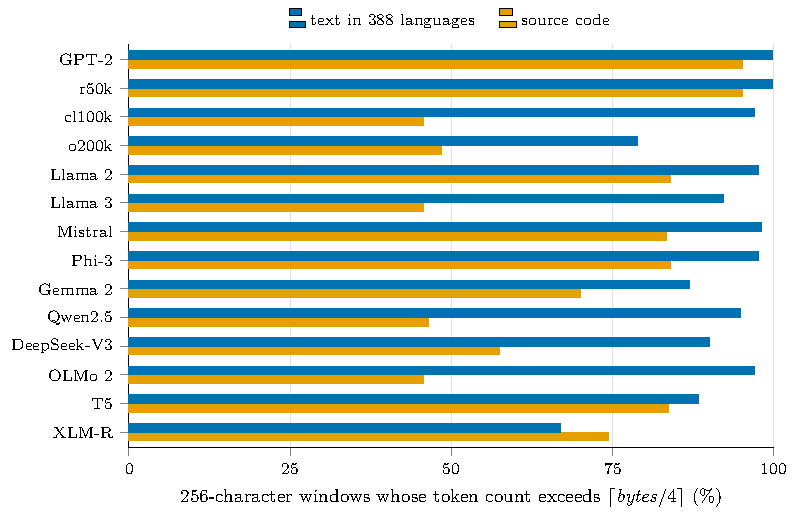
\includegraphics[width=\textwidth]{fig-tokenizers.pdf}
\caption{Share of 256-character windows whose token count exceeds $\lceil\bytes/4\rceil$,
for each of the fourteen tokenizers. The estimate fails on most multilingual text for every
tokenizer, and on almost all source code for the older byte-level encodings (GPT-2,
\code{r50k}) and the SentencePiece tokenizers. The data are those of
\file{bench/results/tokenizers.json}.}
\label{fig:tokenizers}
\end{figure}

These are not new observations about any one tokenizer: that tokenizers charge
languages very unequally is well documented~\cite{petrov2023language}. The point is
their consequence for bounds. A bound assembled from per-part token counts is not a
bound, and neither is one that treats the previous call's output cap as its
response's input cost.

\subsection{Bytes and contracts}\label{sec:contracts}

Bytes add up under concatenation, and they do not depend on the tokenizer. OrchLang
therefore computes each request's length in bytes, as the template's bytes plus the
byte bound of each argument, and converts to tokens once per request, through a
contract for the model's tokenizer.

\begin{definition}[Tokenizer contract]\label{def:contract}
A tokenizer $\tau$ satisfies the \emph{contract} $(\kappa, \sigma)$ if
$\tau(s) \leq \kappa \cdot \bytes(s) + \sigma$ for every string $s$. Its \emph{expansion}
$\lambda_\tau$ is the largest number of bytes that one vocabulary entry decodes to.
\end{definition}

For a byte-level BPE tokenizer, $\kappa = 1$ and $\sigma = 0$ hold structurally, because
every token covers at least one byte. A SentencePiece tokenizer with byte fallback
needs a small $\sigma$ for its dummy prefix and special tokens. Qwen2.5 needs
$\kappa = 3$, because it tokenizes after NFC normalisation, and Unicode's stability
policy guarantees that normalising a string to NFC never makes it more than three
times longer in UTF-8~\cite[Section 9]{uax15}. T5 and XLM-R have no structural
contract; the compiler lets a workflow name them but warns (\code{W267}) and leaves
the guaranteed bound undefined. \Cref{tab:contracts} lists the contracts, which a
script generates from the measurements; it refuses to emit any contract that a
measurement contradicts.

\begin{table}[t]
\centering
\caption{Tokenizer contracts used by the compiler: $\tau(s) \leq \kappa\cdot\bytes(s) + \sigma$,
and $\lambda$ bytes at most per decoded token. The contracts are structural arguments checked
against exhaustive per-code-point measurements; they are not proofs.}
\label{tab:contracts}
\footnotesize
\begin{tabularx}{\textwidth}{@{}>{\raggedright\arraybackslash}X>{\raggedright\arraybackslash}p{4.4cm}ccc@{}}
\toprule
Tokenizers & Family & $\kappa$ & $\sigma$ & $\lambda$ \\
\midrule
GPT-2, \code{r50k}, \code{cl100k}, \code{o200k}, DeepSeek-V3, OLMo~2 & byte-level BPE & 1 & 0 & 128 \\
Llama~3 & byte-level BPE & 1 & 1 & 128 \\
Qwen2.5 & byte-level BPE after NFC & 3 & 0 & 128 \\
Llama~2, Mistral & SentencePiece BPE, byte fallback & 1 & 2 & 27, 25 \\
Phi-3 & SentencePiece BPE, byte fallback & 1 & 1 & 27 \\
Gemma~2 & SentencePiece BPE, byte fallback & 1 & 1 & 48 \\
T5, XLM-R & SentencePiece Unigram, NFKC-like & \multicolumn{2}{c}{none} & 18, 48 \\
\bottomrule
\end{tabularx}
\end{table}

The byte length of a response of $o$ output tokens is at most $\lambda_\tau \cdot o$,
provided decoding a sequence of tokens, with invalid UTF-8 replaced by U+FFFD, never
yields more bytes than decoding its tokens separately. We checked this property
exhaustively on all byte strings of length at most three and on 300,000 random
pairs, but did not prove it. A model may also declare a client-side byte cap
(\code{max\_bytes}), which then replaces the product.

\begin{theorem}[Guaranteed bound]\label{thm:bound}
Assume that each provider reports at most its model's cap, that each tokenizer
satisfies its contract, that each envelope adds at most the declared overhead, that
each input satisfies its declared byte bound, and that each response has at most
$\lambda \cdot \capm$ bytes, or at most the declared byte cap. Then in every execution
the output tokens and the billed input tokens are at most the certificate's
\code{output\_tokens} and \code{input\_tokens\_guaranteed}, and their sum is at most
its guaranteed total.
\end{theorem}

\begin{proof}
By induction on the command, combining bounds by a sum for sequencing, a
componentwise maximum for a branch (for the total, the maximum of the arms'
totals) and multiplication by $n$ for \code{retry} $n$, since a body runs at most
$n$ times. For a call, the output count is at most the cap by assumption, and the
billed input is $\tau_m(q) + \mathit{env} \leq \kappa \cdot \bytes(q) + \sigma +
\mathit{overhead}$. The quantity $\bytes(q)$ is the template's bytes plus the bytes of
the arguments, each bounded by its literal length, by the input's declaration, or by
the response bound of the previous call. Arithmetic saturates, which only rounds
up, and a saturated bound is rejected.
\end{proof}

The proof is mechanised as \code{unary\_bound} and \code{guaranteed\_bound}, with the
assumptions as hypotheses (\cref{sec:mechanisation}). The contracts and $\lambda$ are
measured, not proved: that $\tau(s) \leq \kappa \cdot \bytes(s) + \sigma$ holds for
\emph{every} string rests on the structural argument, which the per-code-point
measurement checks but cannot establish.

\begin{example}\label{ex:triage-bound}
Take the variant of \cref{fig:triage} with a one-bit budget, which the compiler
accepts. Its first request is at most 28 template bytes plus 4,096 bytes of ticket, so it is billed at most $4{,}124 + 9 = 4{,}133$ input tokens under
\code{o200k\_base}. The second request contains the first response, which may decode to
$128 \times 300 = 38{,}400$ bytes, so its guaranteed input is $31 + 38{,}400 + 9 =
38{,}440$ tokens, while the estimate counts that response as 300 tokens. The
certificate records a guaranteed input bound of 42,573 tokens, against an estimate of
1,341.
\end{example}

The price of soundness is $\lambda$. A response of 4,096 tokens may decode to
512\,KiB, and a chain of calls compounds it. On the real workflows the guaranteed
bound is four times the estimate where requests carry only inputs and up to 128 times
the estimate where they carry earlier responses (\cref{sec:eval-real}). A client-side
byte cap on the model is the practical remedy.
